\section{需求分析}
	本次实验要求设计一个解压缩程序。
	该程序要实现两个功能,首先为压缩任意文件,压缩后的文件包括解压所需的信息和压缩后的文件本体两部分。
	解压功能则需要利用压缩文件所给的信息,将文件内容还原为原来的文件。
\section{概要设计}
	本程序的函数调用关系如下

	\begin{figure}[H]
		\centering
		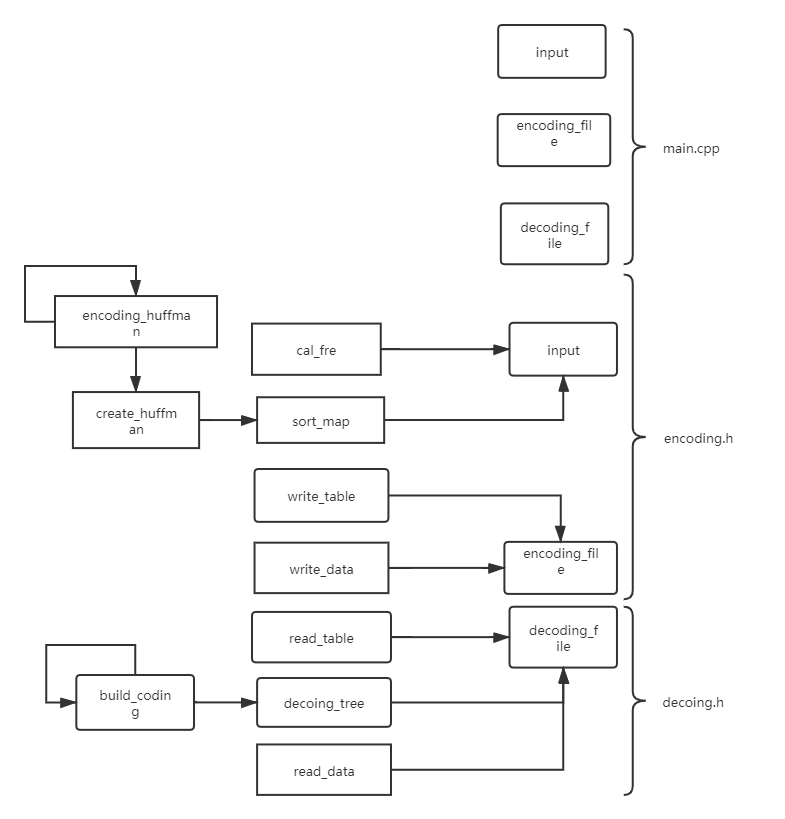
\includegraphics[width=0.5\textwidth]{images/process.png}
		\caption{函数调用关系图}
	 \end{figure}


	 该程序需要用到两个数据结构


	 首先是哈夫曼树
	 \begin{enumerate}
		 \item int flag 该节点是否为叶子结点
		 \item unsigned char val 该节点存有的值
		 \item int fre 该节点的频率
		 \item struct HuffmanTree *ld,*rd 指向左右子树的指针
	 \end{enumerate}


	 再是解压表中元素的表头
	 \begin{enumerate}
		 \item unsigned char size  编码后对应字串的长度
		 \item unsigned char byte  原8位字串
	 \end{enumerate}


	 在压缩后的文件中,文件的结构如下
	 \begin{figure}[H]
		\centering
		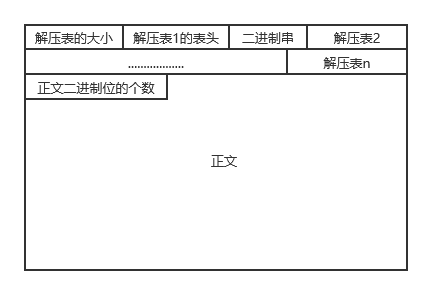
\includegraphics[width=0.5\textwidth]{images/structure.png}
		\caption{文件结构图}
	 \end{figure}


	 每一个解压表由一个表头和一个二进制串构成,表头包含二进制串的长度与二进制串对应字符。

\newpage
	 
\section{详细设计}

\begin{algorithm}[htb] 
	\caption{ HuffmanTree建树 } 
	\label{alg:Framwork} 
	\begin{algorithmic}[1]
	   
		\State 从解码表还原哈夫曼树
	    \Function {build\_decoding}{node, i, s}
			\If{s为空}
				\State 初始化node为值为i的叶子结点
			\EndIf
			\If{s[0] == 0}
				\State s前进一位
				\State 初始化node->ld
				\State build\_decoding{node->ld, i, s}
			\EndIf
			\If{s[0] == 1}
				\State s前进一位
				\State 初始化node->rd
				\State build\_decoding{node->rd, i, s}
			\EndIf
		\EndFunction
		
		\State 利用优先队列建立哈夫曼树
		\Function{create\_huffman}{}
			\While{优先队列中还有一个以上的元素}
				\State 从优先队列中取出两个哈夫曼树
				\State 将两个哈夫曼树合并后放回优先队列
			\EndWhile
		\EndFunction
	\end{algorithmic} 
\end{algorithm}

\newpage

\begin{algorithm}[htb] 
	\caption{ 建立压缩表 } 
	\label{alg:Framwork} 
	\begin{algorithmic}[1]
		\State 利用哈夫曼树建立压缩表
		\Function{encoding\_tree}{rt, str}
			\If{rt是一个叶子结点}
				\State table[rt->val] = str
				\State 二进制位的总数加上$ str.length() * rt->fre $
			\EndIf
			\If{rt的左子树不为空}
				\State encoding\_tree(rt->ld, str + 0)
			\EndIf
			\If{rt的右子树不为空}
				\State encoding\_tree(rt->rd, str + 1)
			\EndIf
		\EndFunction
	\end{algorithmic} 
\end{algorithm}

\newpage


\begin{algorithm}[htb] 
	\caption{ 压缩文件的流程 } 
	\label{alg:Framwork} 
	\begin{algorithmic}[1]
	   \State 调用input()正文信息,调用calu\_fre()统计频率
	   \State 利用得到的频率初始化叶子结点,调用sort\_map(),将叶子结点压入优先队列中
	   \State 调用create\_huffman()建立哈夫曼树,并且调用encoding\_tree()得到压缩表
	   \State 将压缩表以解压表的格式写入文件中
	   \State 统计正文的字节数,值放在size中
	   \State 将size写入文件中
	   \While{$ 128 \leq size $}
			\State size减去128,并读取128个字符存入到line中
			\State 调用write\_data(line),将128压缩后写入文件中
	   \EndWhile
	   \State 将剩下的字符单个读取,并压缩写入文件中
	\end{algorithmic} 
\end{algorithm}

\begin{algorithm}[htb] 
	\caption{ 解压文件的流程 } 
	\label{alg:Framwork} 
	\begin{algorithmic}[1]
	   \State 调用read\_table()读入解压表
	   \State decoding\_tree(),将解压表转为哈夫曼树,便于解压
	   \State 读入正文二进制位的个数
	   \State 调用read\_data(),读入数据并解压写入到文件中
	\end{algorithmic} 
\end{algorithm}

\newpage

\section{调试分析报告}

在压缩算法中我们使用了优先队列算法建树,此处的算法复杂度为$O(klogk)$,然后我们再将正文压缩,复杂度为$O(n)$
所以压缩算法的复杂度为$O(klogk + n)$,其中n为正文的长度,k为正文中出现字符的种类,一般认为n远大于k,则算法复杂度可以视为$O(n)$


解压算法的复杂度为文件大小,即也为$O(n)$

\section{用户使用说明}

用户可以使用IDE或者手动编译源代码stack.cpp,获得可执行文件。

笔者使用的gcc版本为8.1.0


开始程序后,用户需要输入两个参数,0表示压缩,1表示解压。

在压缩模式下,程序会将当前文件夹下的data文件压缩到encoding\_file中。

在解压模式下,程序会将当前文件夹下的encoding\_file文件解压到decoding\_file中。

\section{测试结果}
	为了测试程序压缩的效果和正确性,我们从互联网上下载了《斗破苍窘》,文件大小为8,815KB。
	经我们的程序压缩后,大小为6,494KB,压缩为原来的1/4。

	\begin{figure}[H]
		\centering
		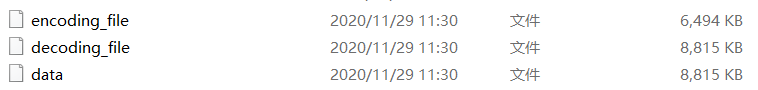
\includegraphics[width=0.5\textwidth]{images/effect.png}
		\caption{压缩效果}
	\end{figure}

	然后再将压缩后的文件解压,得到的文件与原文件对比相同。